\documentclass[a4paper, 12pt]{article}
\usepackage[T2A]{fontenc}
\usepackage[utf8]{inputenc}
\usepackage[english,russian]{babel}
\usepackage{amsmath, amsfonts, amssymb, amsthm, mathtools, misccorr, indentfirst, multirow}
\usepackage{wrapfig}
\usepackage{graphicx}
\usepackage{subfig}
\usepackage{adjustbox}
\usepackage{pgfplots}

\usepackage{geometry}
\geometry{top=20mm}
\geometry{bottom=20mm}
\geometry{left=20mm}
\geometry{right=20mm}
\newcommand{\angstrom}{\textup{\AA}}
\begin{document}
	\begin{titlepage}
		\begin{center}
		МИНИСТЕРСТВО ОБРАЗОВАНИЯ И НАУКИ РОССИЙСКОЙ ФЕДЕРАЦИИ\\
		\footnotesize{Московский физико-технический институт}\\
		\footnotesize{(государственный университет)}\\
		\footnotesize{Кафедра вакуумной электроники}\\
		\vfill
		{\LARGE
		\textbf{Автоэлектронная эмиссия}\\
		}
		\vspace{1cm}
		Лабораторная работа по курсу\\
		вакуумная электроника
		\vfill
		\begin{flushright}
			Выполнил: студент 654гр.\\
			Нехаев А.С.
		\end{flushright}
		\vfill
		г. Долгопрудный\\
		2018 год
		\end{center}
	\end{titlepage}
	\newpage
	\pagenumbering{arabic}
	\tableofcontents
	\newpage
	\section{Цель работы}
	\begin{enumerate}
		\item Изучить работу вакуумной камеры;
		\item Изучить метод получения автоэмиссионного катода с помощью травления пучка углеродных волокон коронным разрядом;
		\item Исследовать автоэмиссионные свойства катода из углеродных волокон и причины нестабильности автоэмиссионного тока в нем.
		\item Снять вольтамперную характеристику;
		\item Построить вольтамперную характеристику в координатах $I(U)$ и в координатах Фаулера-Нордгейма.
	\end{enumerate}
	\newpage
	\section{Теоретическая часть}
	\subsection{Теория автоэлектронной эмиссии металлов}
	При наличии электрического поля над поверхностью металла наблюдается внешняя автоэлектронная эмиссия (автоэмиссия, холодная эмиссия, туннельная эмиссия).\par
	Автоэлектронная эмиссия является эмиссией, не требующей возбуждения электронов. Суть явления состоит в туннелировании электронов сквозь потенциальный барьер на поверхности тела. Такое туннелирование становится возможным за счет искривления потенциального барьера при приложении внешнего поля. При этом появляется область пространства вне тела, в которой электрон может существовать с той же полной энергией, которой он обладает, находясь в теле. Таким образом, автоэлектронная эмиссия обусловлена волновыми свойствами электронов.\par
	Впервые такое объяснение автоэмиссии было предложено в 1928 году Фаулером и Нордгеймом. Ими впервые была получена формула, описывающая взаимосвязь плотности автоэлектронного тока $j$ с напряженностью электрического поля $E$
	\begin{equation}
		j=\frac{e^3}{4\pi^2\hbar}\cdot\frac{E^{1/2}_f}{W_a\varphi^{\frac{1}{2}}}\cdot E^2\cdot\exp\left(-\frac{4}{3e}\frac{\sqrt{2m}}{\hbar}\cdot\frac{\varphi^{\frac{3}{2}}}{E} \right),
	\end{equation}
	где $\varphi=W_a-E_f$ -- работа выхода, $E_f$ -- энергия Ферми, $W_a$ -- уровень вакуума (все энергии отсчитываются от дна зоны проводимости).\par
	Эта формула получена для полубесконечного металла с плоской поверхностью, подчиняющегося модели Зоммерфельда и находящегося при температуре $T=0$ K. При выводе этой формулы Фаулер и Нордгейм предположили, что потенциальный барьер на поверхности тела имеет следующий вид: кривые $А$ и $В$. Позднее в 1929 году Нордгейм предложил ввести в рассмотрение силы электростатического изображения (кривые $C$ и $D$). Это привело к выражениям:
	\begin{equation}
		j=\frac{A'E^2}{\varphi}\cdot e^{-\frac{B'\cdot \varphi^{\frac{3}{2}}\theta(y)}{E}},	
	\end{equation}
	\begin{figure}
		\centering
		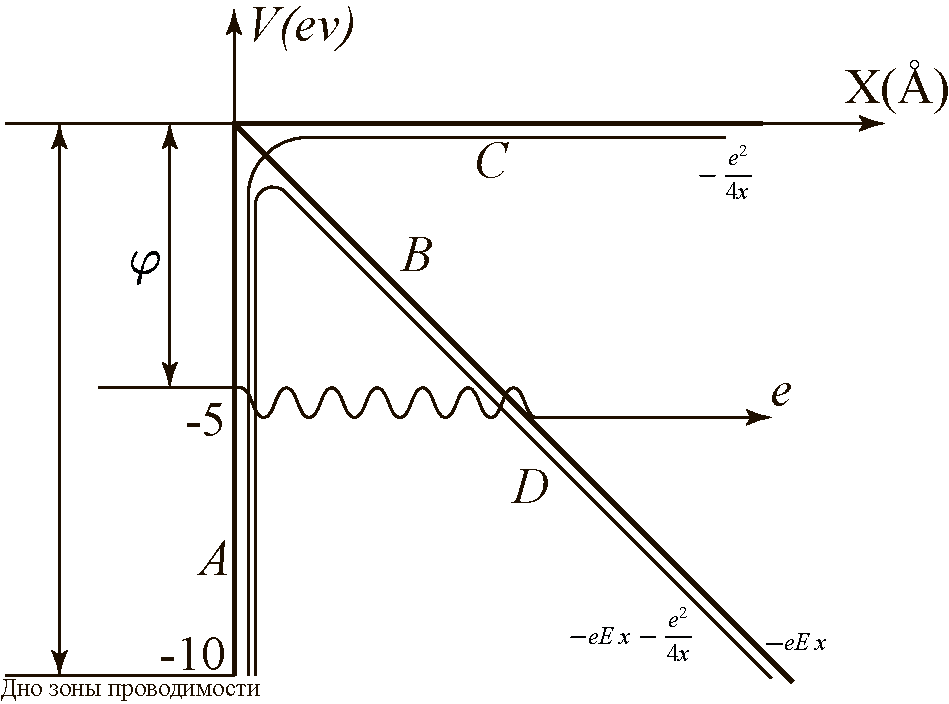
\includegraphics[scale=0.5]{ill.pdf}
		\caption{Поверхностный потенциальный барьер на границе металл-вакуума в присутствие сильного электрического поля. Волнистой линией показан эффект туннелирования электронов сквозь барьер.}
	\end{figure}
	где $A\equiv\frac{e^3}{16\pi^2\hbar}$, $B\equiv\frac{4}{3e}\frac{\sqrt{2m}}{\hbar}$. $\theta(y)$ -- спецфункция, которая была табулирована Нордгеймом, и получила название «функция Нордгейма». При не очень близких к 0 или 1 значениях аргумента функция Нордгейма хорошо приближается аналитическим выражением $\theta(y)=0.965-0.739y^2$. Подставив это в вышеприведённую формулу, получим:
	\begin{equation}
		j=\frac{A'E^2}{\varphi}\cdot e^{-\frac{B'\cdot \varphi^{\frac{3}{2}}}{E}}	\end{equation}
	где $A'=\frac{e^3}{8\pi h}e^{0.739\cdot\frac{\frac{8\pi}{3e}\left(2m\varphi^3\right)^{\frac{1}{2}}}{hE}}$, $B'=0.965\cdot\frac{\frac{8\pi}{3e}\left(2m\varphi^3\right)^{\frac{1}{2}}}{hE}$, $y\equiv\frac{\sqrt{e^3E}}{\varphi}$, $\alpha$ -- угол наклона получившейся кривой.\par
	Строго говоря, теория Фаулера-Нордгейма применима только при температуре $T=0$K. Однако, так как незначительное увеличение температуры мало меняет распределение электронов в металле, лишь размывая его на величину порядка kT вблизи уровня Ферми, то выводы теории остаются качественно верны при температурах, определяемых условием $kt\ll\varphi$. При комнатной температуре, например, $kT=2.6\cdot10^{-2}$ эВ, в то время как характерное значение работы выхода $\varphi=3...6$ эВ.\par
	Если построить график зависимости $\ln \left(\frac{j}{E^2} \right)$ от $\frac{1}{E}$, то соответствующая кривая окажется практически прямой линией в узкой области напряженности поля, которая характерна для типичного автоэмиссионного эксперимента. Эта прямая называется графиком Фаулера-Нордгейма.
	\begin{equation*}
		I=S_{\text{Э}}j
	\end{equation*}
	\begin{equation*}
		E=\beta U
	\end{equation*}
	где $S_{\text{Э}}$ -- площадь поверхности эмиттера, $\beta$ -- форм-фактор острия.\par
	Таким образом, если, с учётом этих формул, построить график $\ln \left(\frac{I}{U^2} \right)$ от $\frac{1}{U}$ то мы получим прямую линию (прямая Фаулера-Нордгейма для полного тока и напряжения). Тангенс угла наклона этой прямой будет определяться выражением:
	\begin{equation}
		\tan(\alpha)=-0.683\cdot\frac{\varphi^{\frac{3}{2}}}{\beta}\cdot\left(3.79\cdot\frac{\sqrt{\beta U}}{\varphi} \right)
	\end{equation}
	$s(y)$ в узкой области напряжённости поля можно считать константой. В рабочем диапазоне токов и напряжений, эту функцию можно приближённо считать равной 1. Тогда
	\begin{equation}
		\tan(\alpha)=-0.683\cdot\frac{\varphi^{\frac{3}{2}}}{\beta},
	\end{equation}
	\subsection{Нестабильность автоэмиссионного тока}
	Основные причины нестабильности тока автоэлектронных катодов следующие:
	\begin{enumerate}
		\item Разрушение поверхности под действием ионной бомбардировки ионами остаточных газов, что может приводить к изменению микрогеометрии поверхности катода: размеров центров и межцентровых расстояний, а также к разрушению центров и изменению межэлектродного расстояния.
		\item Адсорбция и десорбция атомов остаточных газов, которая может вызывать изменение локальной работы выхода катода.
		\item Разрушение или изменение геометрии эмиссионных центров под действием пондеромоторных нагрузок.
		\item Разрушение эмиссионных центров из-за нарушения теплового режима катода при больших плотностях отбираемого тока.
		\item Механическая непрочность катода, приводящая к взаимному смещению элементов катода за счет электростатического отталкивания, и, как следствие, к изменению конфигурации электрического поля.
	\end{enumerate}
	\subsection{Автоэмиссионные свойства углеродных материалов}
	Среди известных углеродных материалов наиболее подходящими для создания АЭК, работающих в условиях высокого вакуума, оказались графит и так называемые полиакрилонитрильные углеродные волокна.\par
	Для уменьшения влияния электростатических сил, отклоняющих периферийные волокна пучка, необходимо придать пучку геометрическую форму, которая позволила бы обеспечить наиболее одинаковое электрическое поле у волокон в пучке. Для этого применяется метод травления коронным разрядом на воздухе.\par
	Действие коронного разряда на углеродные волокна заключается в том, что за счёт бомбардировки катода ионами кислорода O2 происходит окисление углерода C и тем самым стравливание материала катода. Таким образом, длина отдельного волокна, выступающего из пучка волокон, уменьшается до тех пор, пока фактор усиления электрического поля не станет меньше или одинаковым по сравнению с другими волокнами из пучка.
	\section{Техника эксперимента}
	\begin{figure}[!htb]
		\centering
		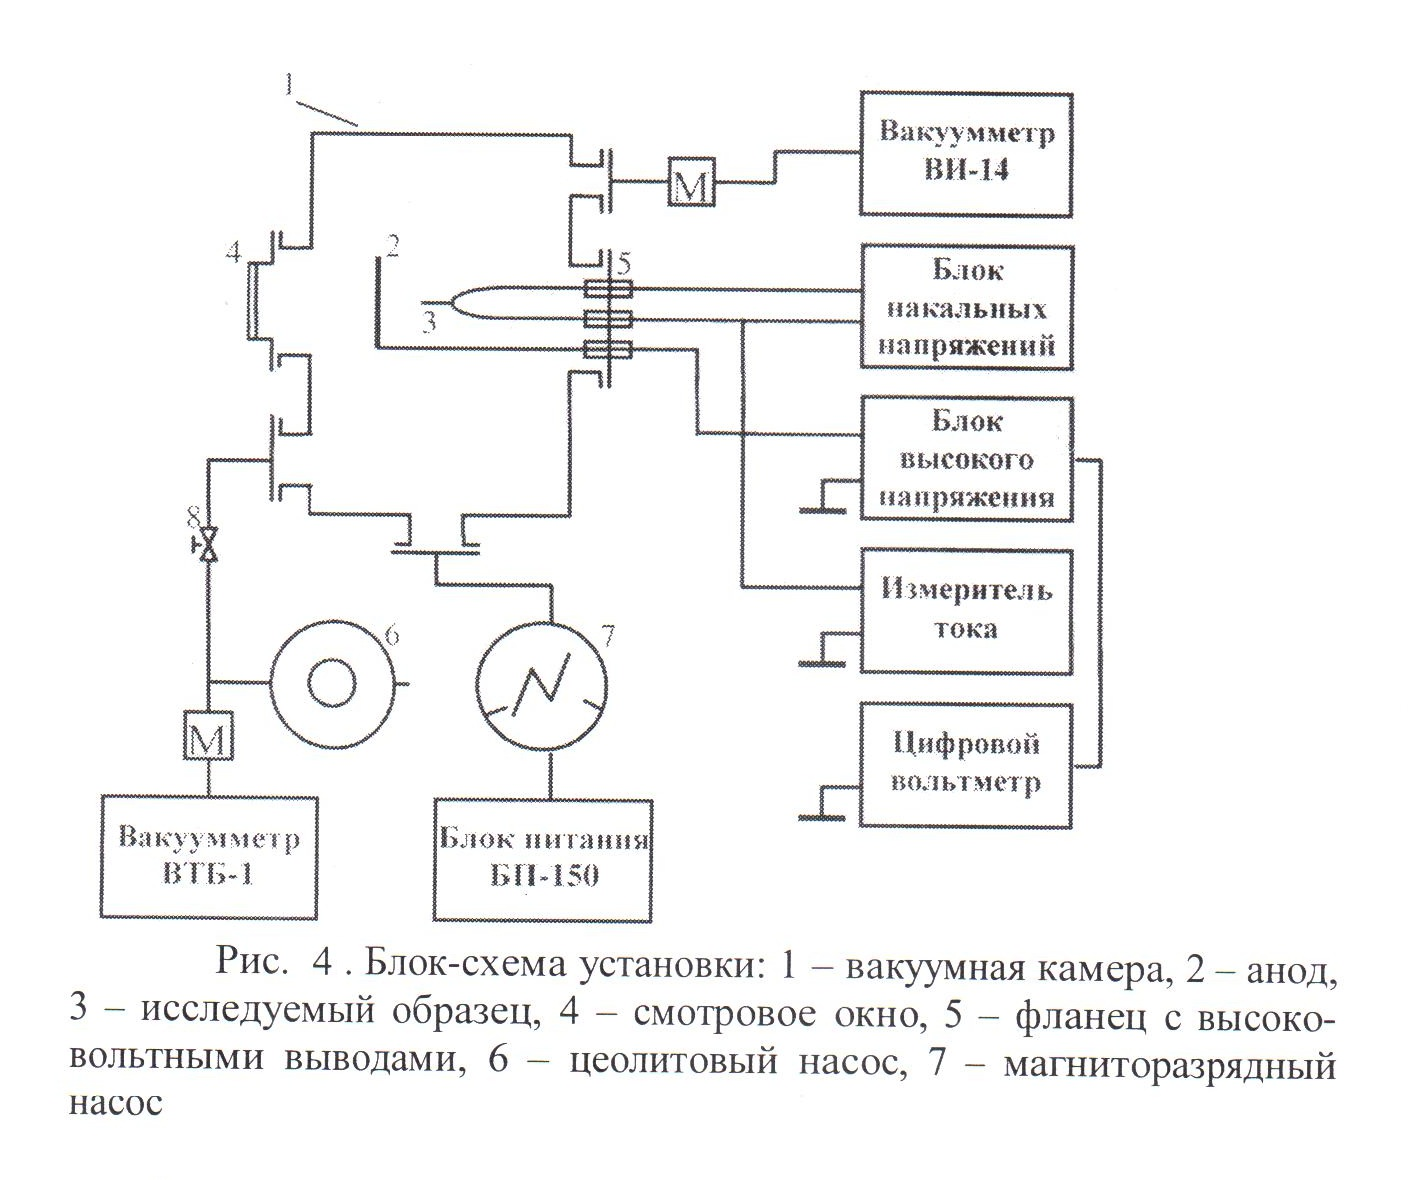
\includegraphics[scale=0.8]{scheme.jpg}
		\caption{Схема лабораторной установки}
	\end{figure}
	В качестве катода выступал пучок углеродных волокон, стравленный предварительно коронным разрядом, в результате электрическое поле для всех волокон пучка было почти одинаковым. Исследуемые автокатоды находились в отпаянной стеклянной лампе. На анод подавалось высокое напряжение, а катод заземлялся.
	\newpage
	\section{Практическая часть}
	\begin{enumerate}
		\item Сняли зависимость автоэмиссионного тока катода из углеродных трубок от приложенного напряжения
		\begin{figure}[!htb]
			\centering
			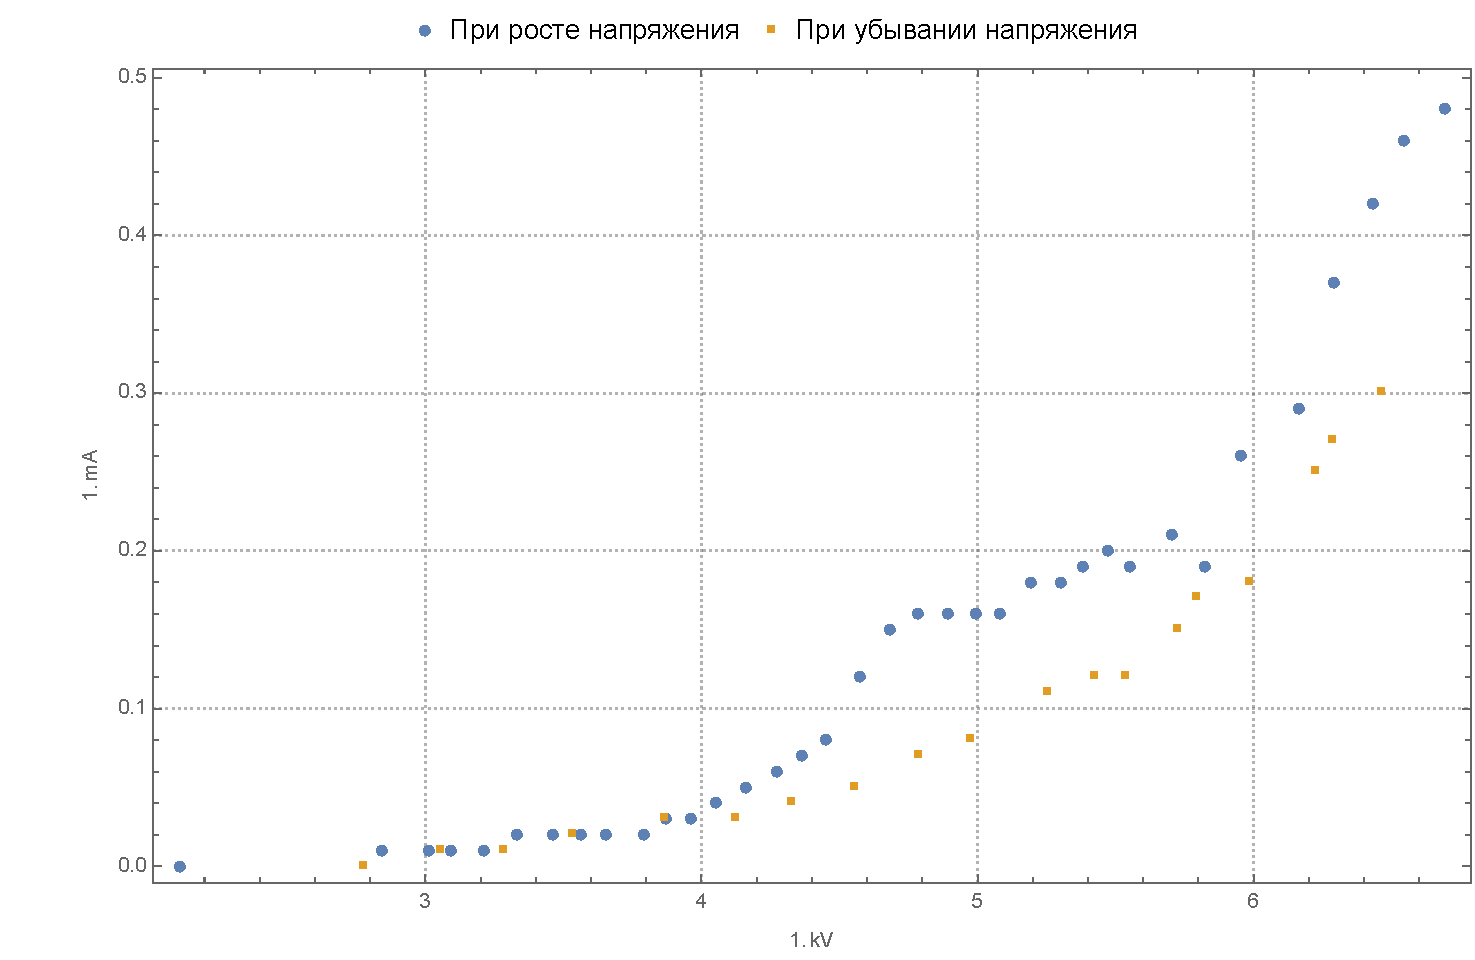
\includegraphics[scale=0.5]{fig1.pdf}
			\caption{График зависимости автоэмиссионного тока от напряжения}
		\end{figure}
		\\
		По графику можно определить, что ВАХ системы отличалась при возрастании и убывании напряжения.
		\item Построили полученную зависимость в координатах Фаулера-Нордгейма
		\begin{figure}[!htb]
			\centering
			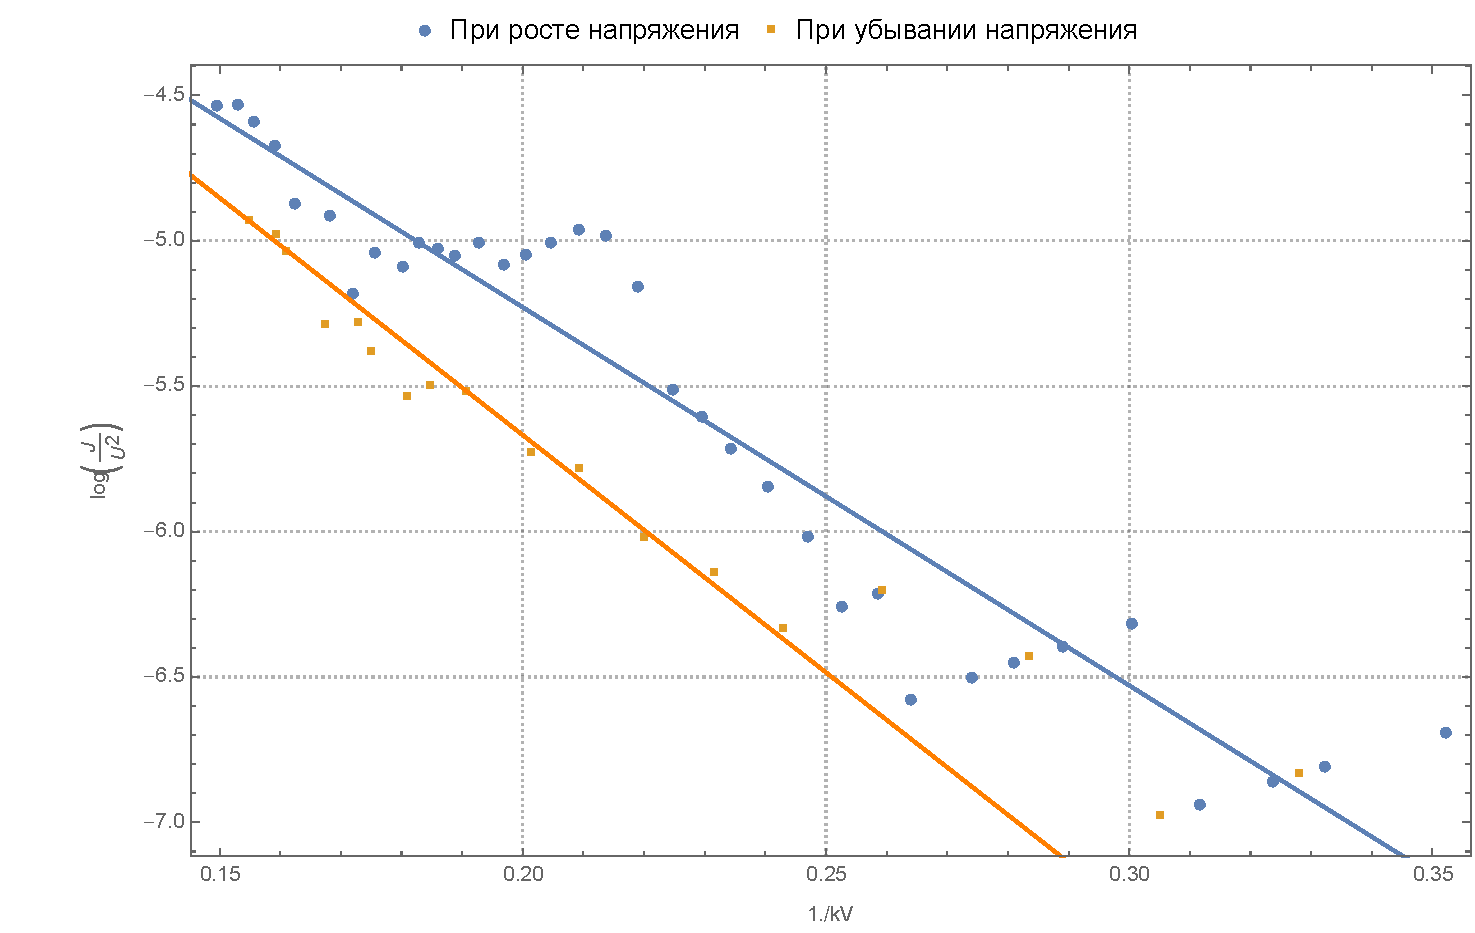
\includegraphics[scale=0.55]{fig2.pdf}
			\caption{График зависимости давления от времени}
		\end{figure}\\
		По полученным кривым можно выяснить, что основную роль в нестабильности тока имело изменение размеров эмиссионных центров, так как значение величины А + 2ln(B), где А – смещение кривой ФН, а B - её коэффициент наклона, осталось почти постоянным в  течение снятия ВАХ.\par
		Форм фактор для возрастания и убывания соответственно равен $\beta=-\frac{0.683\varphi^{\frac{3}{2}}}{\tan(\alpha)}$
	\end{enumerate}
	\newpage
	\section{Вывод}
	\begin{enumerate}
		\item Изучили особенности автоэлектронной эмиссии и её применения.
		\item Ознакомились с техникой автоэлектронной микроскопии и областями её применения, а также методикой получения острий для автоэмиссионных микроскопов
		\item Исследовали автоэмиссионные свойства катода из углеродных волокон и определили причину нестабильности автоэмиссионного тока такого катода.
	\end{enumerate}
\end{document}